\documentclass{article}
\usepackage{nmm}

\title{Strong Normalization from Weak Normalization in Non-Dependent Pure Type Systems via Thunkification}
\author{Nathan Mull}

\begin{document}

\maketitle

\abstract{
In this report, I present a generalization of Xi's thunkification translation \cite{xi-1997} to a class of non-dependent pure type systems, in analogy with the generalization of S{\o}rensen's CPS translation \cite{sorensen-1997} by Barthe \etal \cite{barthe-et-al-2001}.
The primary benefit of this result, as with Xi's original translation, is that its proof is quite a bit simpler than its CPS-based counterpart.
As a further simplification, I also present the class of \textit{tiered} pure type systems, which are concretely specified, and so simpler to work with than the systems considered by Barthe \etal and others, but are equivalent with respect to questions regarding normalization.
}

\section{Introduction}

Pure type systems were introduced by Terlouw \cite{terlouw-1989}, Berardi \cite{berardi-1988}, and later by Barendregt \cite{barendregt-1991, barendregt-1993}, as a natural generalization of the lambda cube; they include the lambda cube as well as systems with more complex sort structure and product type formation.
The study of pure type systems can in some sense be viewed as the study of how sort structure affects the meta-theoretic properties of a type system, especially because of the minimal set of type formers (\eg, there are no $\Sigma$-types).
One such meta-theoretic property, arguably one of the most important, is normalization.
A type system is \textit{weakly normalizing} if every typable term has a normal form and is \textit{strongly normalizing} if no typable term appears in an infinite reduction sequence.
Girard \cite{girard-1972} demonstrated that sort structure can have a nontrivial effect on the normalization behavior of a type system by showing that the pure type system $\lambda U$ is not strongly normalizing, the import being that circularity in the sort structure of a pure type system is not a necessary condition for non-normalization.
This leaves open the problem of understanding the interplay of sort structure and normalization.
One particular open question that has persisted is the Baredregt-Geuvers-Klop conjecture, which states that weak normalization implies strong normalization for all pure type systems.

The primary technique for proving strong normalization from weak normalization passes through some form of the $\lambda I$-calculus, where it readily follows from a conservation theorem along the lines of the one proved by Church and Rosser for the untyped lambda calculus \cite{church-rosser-1936}.
The argument is roughly as follows:
Suppose a system $\lS$ is weakly normalizing.
Define a translation from expressions to $\lambda I$-expressions in $\lS$ which preserve infinite reduction paths.
The translated terms are weakly normalizing and, hence, are strongly normalizing by the conservation theorem.
And since the translation preserves infinite reduction paths, the untranslated terms are themselves strongly normalizing.

This technique was originally used by S{\o}rensen \cite{sorensen-1997} via continuation-passing (CPS), and Xi \cite{xi-1997} subsequently presented an alternative proof via thunkification that is arguably simpler; rather than passing around continuations, expressions are thunked and the unit term which is passed along to evaluate thunks is padded with sub-expression information necessary to translate to $\lambda I$-expressions.
Barthe \etal \cite{barthe-et-al-2001} generalized S{\o}rensen's result to a class of non-dependent pure type systems which includes non-normalizing systems like $\lambda U$.
This report contains the analogous generalization for Xi's thunkification translation, with the hope of providing a simpler, more approachable proof of the main result of the Barthe \etal that may present opportunities for further improvements.

In the interest of further simplification, I also present a class of basic, concrete pure type systems I call \textit{tiered} pure type systems.
Despite their simplicity they are sufficient to consider with regards to questions about normalization behavior if we want to derive the same result as the one by Barthe \etal
Tiered pure type systems can be viewed as the \textit{atoms} of persistent stratified systems, \ie, the persistent stratified systems are disjoint unions of tiered systems.

In what follows I present some preliminary material, which includes some exposition on tiered systems.
I then present the generalized thunkification translation in two parts: one part for the type-level translation and one part for term-level translation.
Finally, I show how to derive strong normalization from weak normalization with this translation.

\section{Preliminaries}

A pure type system is specified by a triple of sets $(\sorts, \axioms, \rules)$ satisfying $\axioms \subset \sorts \times \sorts$ and $\rules \subset \sorts \times \sorts \times \sorts$.
The elements of $\sorts$, $\axioms$, and $\rules$ are called sorts, axioms and rules, respectively.
We use $s$ and $t$ as a meta-variable for sorts.\footnote{For any subsequent meta-variables, we also allow positive integer subscripts and tick marks, \eg, $s_1$, $s_2$, and $s'$. Note, however, that in later sections, $s_i$ will refer to a particular sort in tiered systems. We will try to be as clear as possible when distinguishing between these two cases of notation.}

For each sort $s$, fix a $\mathbb Z^+$-indexed set of expression variables $\vars_s$.
Let $\var[s]{v_i}$ denote the $i$th expression variable in $\vars_s$ and let $\vars$ denote $\bigcup_{s \in \sorts} \vars_s$.
We use $x$, $y$, and $z$ as meta-variables for expression variables.
The choice to annotate variables with sorts is one of convenience.
The annotations can be dropped for the systems we consider, and are selectively included in the exposition.

The set of expressions of a pure type system with sorts $\sorts$ is described by the grammar
\[
\terms \bnfeq
    \sorts \sbar
    \vars \sbar
    \PiT \vars \terms \terms \sbar
    \lambdaT \vars \terms \terms \sbar
    \terms \terms
\]
We use $M$, $N$, $P$, $A$, $B$, and $C$ as meta-variables for expressions.
Free variables, bound variables, $\alpha$-congruence, $\beta$-reduction, substitution, \etc are defined as usual (see, for example, Barendregt's presentation \cite{barendregt-1993}).
Substitution of $x$ with $N$ in $M$ is denoted $\sub M N x$.

A \term{statement} is a pair of expressions, denoted $\statement M A$.
The first expression is called the \term{subject} and the second is called the \term{predicate}.
A \term{proto-context} is a sequence of statements whose subjects are expression variables.
We call these statements appearing in proto-contexts \term{declarations}.
We use $\Gamma$, $\Delta$, and $\Upsilon$ as meta-variables for contexts.
Often the sequence braces of contexts are dropped and concatenation of contexts is denoted by comma-separation.
The $\beta$-equality relation and substitution extend to contexts element-wise.
For a context $\Gamma$ and statement $(\statement x A)$ we write $(\statement x A) \in \Gamma$ if that statement appears in $\Gamma$.
We define the subset relation $\Gamma \subset \Delta$ for contexts $\Gamma$ and $\Delta$ analogously.

A \term{proto-judgment} is a proto-context together with statement, denoted $\judgment \Gamma M N$.
The designation ``judgment" is reserved for proto-judgments that are derivable according to the rules below.
Likewise, the designation ``context" is reserved for proto-contexts that appear in some (derivable) judgment.\footnote{Alternatively, in any non-trivial pure type system $\lambda S$, a proto-context $\Gamma$ is a context if $\judgment \Gamma s {s'}$ for any axiom $(s, s')$.}

\begin{definition}
The pure type system $\lambda S$ specified by $(\sorts, \axioms, \rules)$ has the following rules for deriving judgments.
In what follows, the meta-variables $s$ and $s'$ range over all sorts in $\mathcal S$ when unspecified.
We say that a variable $\avar s x$ is \term{fresh} with respect to a context $\Gamma$ if it does not appear anywhere in $\Gamma$.

\begin{itemize}
\item
\textbf{Axioms.} For any axiom $(s, s')$
\[
    \judgment[\lS] {} {s} {s'}
\]

\item
\textbf{Variable Introduction.} For a fresh variables $\avar s x$
\begin{prooftree}
\AxiomC {$
\judgment[\lS] \Gamma A s
$}

\UnaryInfC {$
    \judgment[\lS] {
        \Gamma, \statement {\avar s x} A
    }{
        \avar s x
    }{
        A
    }
$}
\end{prooftree}

\item
\textbf{Weakening.} For a fresh variable $\avar s x$
\begin{prooftree}
\AxiomC {$
    \judgment[\lS] \Gamma M A
$}
\AxiomC {$
    \judgment[\lS] \Gamma B s
$}
\BinaryInfC {$
    \judgment[\lS] {\Gamma, \statement {\avar s x} B} M A
$}
\end{prooftree}
	
\item
\textbf{Product Type Formation.} For any rule $(s, s', s'')$
\begin{prooftree}
\AxiomC {$
    \judgment[\lS] \Gamma A {s}
$}
\AxiomC {$
    \judgment[\lS] {\Gamma, \statement {\avar {s} x} A} B {s'}
$}
\BinaryInfC {$
    \judgment[\lS] \Gamma {\PiT {\avar s x} A B} {s''}
$}
\end{prooftree}

\item
\textbf{Abstraction.}
\begin{prooftree}
\AxiomC {$
    \judgment[\lS] {\Gamma, \statement {\avar s x} A} M B
$}
\AxiomC {$
    \judgment[\lS] \Gamma {\PiT {\avar s x} A B} {s'}
$}
\BinaryInfC {$
    \judgment[\lS] \Gamma {\lambdaT {\avar s x} A M} {\PiT {\avar s x} A B}
$}
\end{prooftree}

\item
\textbf{Application.}
\begin{prooftree}
\AxiomC {$
    \judgment[\lS] \Gamma M {\PiT {\avar s x} A B}
$}
\AxiomC {$
    \judgment[\lS] \Gamma N A
$}
\BinaryInfC {$
    \judgment[\lS] \Gamma {M N} {\sub{B}{N}{\avar s x}}
$}
\end{prooftree}

\item
\textbf{Conversion.} For any terms $A$ and $B$ such that $A \eqbeta B$
\begin{prooftree} \AxiomC {$
    \judgment[\lS] \Gamma M A
$}
\AxiomC {$
    \judgment[\lS] \Gamma B s
$}
\BinaryInfC {$
    \judgment[\lS] \Gamma M B
$}
\end{prooftree}
\end{itemize}
\end{definition}

The subscript on the turnstile is dropped when there is no fear of ambiguity.
The annotations on variables in $\Pi$-expressions and $\lambda$-expressions are non-standard, and will in most cases be dropped, but they affect the statement of the generation lemma (\Autoref{lem:generation}).
It is also standard to write $A \to B$ for $\PiT x A B$ in the case that $x$ does not appear free in $B$, and to use the derived inference rule 
\begin{prooftree}
\AxiomC {$
    \judgment[\lS] \Gamma A {s}
$}
\AxiomC {$
    \judgment[\lS] {\Gamma} B {s'}
$}
\BinaryInfC {$
    \judgment[\lS] \Gamma {A \to B} {s''}
$}
\end{prooftree}

An expression $M$ is said to be \textbf{derivable} in $\lS$ if there is some context $\Gamma$ and expression $A$ such that $\judgment[\lS] \Gamma M A$.
Although there is no distinction between terms and types, it is useful to call a judgment a \textbf{type judgment} if it is of the form $\judgment \Gamma A s$ where $s \in \sorts$, and a \textbf{term judgment} if it is of the form $\judgment \Gamma M A$ where $\judgment \Gamma A s$ for some sort $s$.
We also say that $M$ is a term and $A$ is a type.
By type correctness (\Autoref{lem:type-correctness}), a judgment that is not a type judgment is a term judgment, though some judgments are both type and term judgments.
In the system specified by $(\{s_1, s_2\}, \{(s_1, s_2)\}, \emptyset)$, for example,
\begin{itemize}
    \item $\judgment {} {s_1} {s_2}$ is a type judgements but not a term judgment,
    \item $\judgment {\statement x {s_1}} x {s_1}$ is a type judgment and a term judgment, and
    \item $\judgment {\statement x {s_1}, \statement y x} y x$ is a term judgment but not a type judgment.
\end{itemize}

\subsection{Meta-Theory}

We collect here the meta-theoretic lemmas necessary for the subsequent results.
I choose not to present any proofs, and instead refer the reader to any of the great resources on pure type systems (\cite{barendregt-1993, barthe-et-al-2001, kamareddine-et-al-2004}, among others).
For the remainder of the section, fix a pure type system $\lS$.

\begin{lemma}
\label{lem:generation}
(Generation)
For any context $\Gamma$ and expression $A$, the following hold.
\begin{itemize}
\item \underline{Sort.} For any sort $s$, if $\judgment \Gamma s A$, then there is a sort $s'$ such that $A \eqbeta s'$ and $(s, s') \in \axioms$.
\item \underline{Variable.} For any sort $s$ and variable $\avar s x$, if $\judgment \Gamma {\avar s x} A$, then there is an type $B$ such that $\judgment \Gamma B s$ and $(\statement {\avar s x} B)$ appears in $\Gamma$ and $A \eqbeta B$.
\item \underline{$\Pi$-expression.} For any sort $s$ and expressions $B$ and $C$, if
\[
    \judgment \Gamma {\PiT {\avar s x} B C} A
\]
then there are sorts $s'$, and $s''$ such that
\[
    \judgment \Gamma B s \qquad \text{and} \qquad \judgment {\Gamma, \statement {\avar s x} B} C {s'}
\]
and $(s, s', s'') \in \rules$ and $A \eqbeta s''$.
\item \underline{$\lambda$-expression.} For any sort $s$ and expressions $B$ and $M$, if
\[
\judgment \Gamma {\lambdaT {\avar s x} B M} A
\]
then there is a type $C$ and sort $s'$ such that such that
\[
\judgment \Gamma {\PiT {\avar s x} B C} {s'} \qquad \text{and} \qquad \judgment {\Gamma, \statement {\avar s x} B} M C
\]
and $A \eqbeta \PiT {\avar s x} B C$.
\item \underline{Application.} For expressions $M$ and $N$, if $\judgment \Gamma {MN} A$, then there is a sort $s$ and types $B$ and $C$ such that $\judgment \Gamma M {\PiT {\avar s x} B C}$ and $\judgment \Gamma N B$ and $A \eqbeta \sub C N {\avar s x}$.
\end{itemize}
\end{lemma}


\begin{lemma}
\label{lem:substition}
(Substitution)
For contexts $\Gamma$ and $\Delta$ and expressions $M$, $N$, $A$ and $B$, if
\[
    \judgment {\Gamma, \statement x A, \Delta} M B \qquad \text{and} \qquad \judgment \Gamma N A
\]
then
\[
    \judgment {\Gamma, \sub {\Delta} N x} {\sub M N x} {\sub B N x}
\]
\end{lemma}

\begin{lemma}
\label{lem:type-correctness}
(Type Correctness)
For any context $\Gamma$ and expressions $M$ and $A$, if $\judgment \Gamma M A$ then $A \in \sorts$ or there is a sort $s$ such that $\judgment \Gamma A s$.
\end{lemma}

\begin{lemma}
\label{lem:thinning}
(Thinning)
For contexts $\Gamma$ and $\Delta$ and expressions $M$ and $A$, if  $\Gamma \subset \Delta$ and $\judgment \Gamma M A$, then $\judgment \Delta M A$.
\end{lemma}

\begin{lemma}
\label{lem:permutation}
(Permutation) For contexts $\Gamma$ and $\Delta$, variables $x$ and $y$, and expressions $A$, $B$, $M$, and $C$, if $x$ does not appear free in $B$ and
\[
    \judgment{
        \Gamma, \statement x A, \statement y B, \Delta
    }{M}{C}
\]
then
\[
    \judgment{
        \Gamma, \statement y B, \statement x A, \Delta
    }{M}{C}
\]
\end{lemma}

\begin{definition}
\label{def:functional}
A pure type system is \textbf{functional} if
\begin{itemize}
    \item for all axioms $(s, s')$ and $(t, t')$ if $s = t$ then $s' = t'$;
    \item for all rules $(s, s', s'')$ and $(t, t', t'')$ if $s = t$ and $s' = t'$ then $s''  = t''$.
\end{itemize}
\end{definition}

\begin{lemma}
\label{lem:unicity}
(Type Unicity)
If $\lambda S$ is functional then for any context $\Gamma$ and expressions $M$, $A$, and $B$, if $\judgment \Gamma M A$ and $\judgment \Gamma M B$, then $A \eqbeta B$.
\end{lemma}

\begin{definition}
A sort $s$ is a \textbf{top-sort} if there is no sort $s'$ such that $(s, s') \in \axioms$.
\end{definition}

\begin{restatable}{lemma}{lemTopSort}
\label{lem:top-sort}
(Top-Sort Lemma)
For any context $\Gamma$, variable $x$, expressions $A$ and $B$, and top-sort $s$ the following hold.
\begin{enumerate}
    \item $\negjudgment \Gamma s A$
    \item $\negjudgment \Gamma x s$
    \item $\negjudgment \Gamma {AB} s$
    \item $\negjudgment \Gamma {\lambdaT x A B} s$.
\end{enumerate}
\end{restatable}


\subsection{Tiered Pure Type Systems}

General pure type systems are notoriously difficult to work with so it is typical to consider a class of pure type systems satisfying a collection of properties, \eg, functionality, persistence, and stratification, as defined below.
Here I choose to work with an simple class of systems I call \textbf{tiered pure type systems}, which have a very concrete description.

\begin{definition}
Let $n$ be a positive integer.
A pure type system is \textbf{$n$-tiered} if it has the form
\begin{align*}
    \sorts &= \setcomp {s_i} {i \in \upto n} \\
    \axioms &= \setcomp {(s_i, s_{i + 1})} {i \in \upto {n - 1}} \\
    \rules &\subset \{(s_1, s_1, s_1)\} \cup \setcomp {(s, s', s')} {(s, s') \in \sorts \times \sorts}
\end{align*}
\end{definition}

\begin{figure}
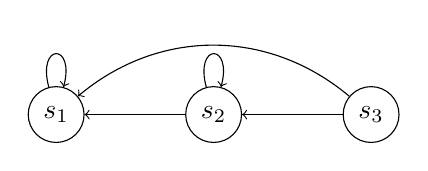
\begin{tikzpicture}
\node[shape=circle,draw=black] (1) at (0,0) {$s_1$};
\node[shape=circle,draw=black] (2) at (2,0) {$s_2$};
\node[shape=circle,draw=black] (3) at (4,0) {$s_3$};
\draw [->] (1) to [loop above] (1);
\draw [->] (2) to [loop above] (2);
\draw [->] (2) -- (1);
\draw [->] (3) -- (2);
\draw [->] (3) to [bend right=40] (1);
\end{tikzpicture}
\centering
\caption{A visual representation of the system $\lambda U$, where an arrow $(s_i, s_j)$ indicates the presence of the rule $(s_i, s_j, s_j)$ (axioms are not represented in the graph except in the ordered the nodes are presented).}
\label{fig:tiered}
\end{figure}

From this point forward, I will freely use the notation $(s, s')$ for the rule $(s, s', s')$.
A couple remarks about these systems:
\begin{itemize}
\item these systems can be envisioned as graphs as in \autoref{fig:tiered};
\item the 2-tiered systems are exactly the lambda cube;
\item the $n$-tiered systems and are considered in passing by Barthes \etal (Remark 2.39, \cite{barthe-et-al-2001}). They include natural subsystems of $\ecc n$ (as defined in \cite{luo-1990}) with only the two-sorted rules.
\end{itemize}
Working in tiered systems simplifies the arguments in the following section because of their explicit structure, and they are sufficient to consider in so far as their normalization is equivalent to that of a previously considered classes of systems defined in terms of less concrete properties.
This is likely a folklore result, as I could not find a reference for it, so I have included the proof here.
First, some standard definitions, along with a couple definitions taken from Barthe \etal \cite{barthe-et-al-2001} for their definition of generalized non-dependent systems.
Note that we have already seen the definition of functional pure type systems (\Autoref{def:functional}) in the previous section.

\begin{definition}
A pure type system is \textbf{persistent} if it is functional and
\begin{itemize}
    \item For all axioms $(s, s')$ and $(t, t')$ if $s' = t'$ then $s = t$;
    \item $\rules \subset \setcomp {(s, s', s')} {(s, s') \in \sorts \times \sorts}$
\end{itemize}
\end{definition}

Let `$\leq_\axioms$' denote the reflexive transitive closure of $\axioms$, and let `$<_\axioms$' be defined as usual (the subscript is dropped when there is no fear of ambiguity).

\begin{definition}
A pure type system is \textbf{weakly stratified} if there is no infinite sequence of sorts $s, s', s'', \dots$ such that
\[
s < s' < s'' < \dots \qquad\text{or}\qquad s > s' > s'' >\dots\footnote{This is a weaker notion of stratification than the one given by Barthe et al.\ \cite{barthe-et-al-2001}, in part because it is decoupled from the notion of non-dependence, and in part because their definition does not account for infinite descending sequences of sorts.}
\]
\end{definition}

In order to state the following equivalence, we work in the structural theory of pure type systems of Roux and van Doorn \cite{roux-doorn-2014} (albeit, not the particularly interesting part of it).

\begin{definition}
For pure type systems $\lambda S$ and $\lambda S'$, the \textbf{disjoint union} $\lambda S \sqcup \lambda S'$ is specified by
\begin{align*}
    \sorts _{\lambda S \sqcup \lambda S'} &\df \sorts _{\lambda S} \sqcup \sorts_{\lambda S'} \\
    \axioms_{\lambda S \sqcup \lambda S'} &\df \axioms_{\lambda S} \sqcup \axioms_{\lambda S'} \\
    \rules _{\lambda S \sqcup \lambda S'} &\df \rules _{\lambda S} \sqcup \rules_{\lambda S'}
\end{align*}
\end{definition}

\begin{lemma}
A pure type system is persistent and weakly stratified if and only if it is the disjoint union of tiered pure type systems.
\end{lemma}

\begin{proof}
It is straightforward to verify that tiered systems are persistent and weakly stratified, and that the same is true for disjoint unions of such systems, so we focus on the other direction.
Let $\lambda S$ be a pure type system that is persistent and weakly stratified and let $T$ denote the set of top-sorts in $\sorts$.
Considered the $T$-indexed partition $\{\sorts_t\}_{t \in T}$ of $\sorts$ where $\sorts_t = \setcomp {s} {s \leq t}$.
We say a \textbf{chain} from $s$ to $s'$ is a sequence of sorts $(\upsilon_1, \dots, \upsilon_k)$ such that $\upsilon_1 = s$ and $\upsilon_k = s'$ and $(\upsilon_i, \upsilon_{i + 1}) \in \axioms$ for each $i$ in $\upto{k - 1}$.
Persistence ensures that each set in this partition is totally ordered by $\leq_\axioms$.
In particular, it is possible to show that there is at most one chain ending at $t$ of any length $n$ contained in a set $\sorts_t$ for a top-sort $t$.
This also implies that each set in the partition is disjoint.
Stratification ensures that each set is finite.
Finally note that the partition covers all of $\sorts$.
If $s$ is not in $\sorts_t$ for some top-sort $t$, then since $s$ is not a top-sort, there is some other sort $s'$ such that $(s, s') \in \axioms$ and $s'$ is not in any set of the partition. This process can iterated to build an infinite ascending sequence of sorts.
So $\{\sorts_t\}_{t \in T}$ is in fact a partition.

Let $\lambda S_t$ denote the pure system specified by
\begin{align*}
\sorts_{\lambda S_t} &\df \sorts_t \\
\axioms_{\lambda S_t} &\df \axioms_{\lambda S} \cap (\sorts_t \times \sorts_t) \\
\rules_{\lambda S_t} &\df \rules_{\lambda S} \cap (\sorts_t \times \sorts_t \times \sorts_t)
\end{align*}
The axioms and rules of each system are clearly pairwise disjoint.
They also cover all axioms and rules of $\lambda S$.
For suppose that $(s, s')$ is an axiom such that $s \in \sorts_t$ and $s' \in \sorts_{t'}$ for distinct top-sorts $t$ and $t'$.
Since $s$ is not a top-sort, there must be some other sort $s''$ in $\sorts_t$ such that $(s, s'') \in \axioms$.
Then persistence implies that $s' = s''$, contradicting disjointness.
The same kind of argument applies for the rules.
Finally, the fact that each $\sorts_t$ is totally ordered with respect to $\leq_\axioms$ and is finite implies that each system $\lambda S_t$ is tiered.
Therefore, we can view $\lambda S$ as the system $\bigsqcup_{t \in T} \lambda S_t$.
Formally, they are isomorphic pure type systems.\footnote{The definition of a pure type system homomorphism is as one might expect, see \cite{roux-doorn-2014} for more details.}
\end{proof}

This fact can be easily lifted to generalized non-dependent systems.

\begin{definition}
A pure type system $\lS$ is \textbf{generalized non-dependent} if it is persistent and weakly stratified and its rules are non-dependent, \ie, if $(s, s') \in \rules_{\lS}$ then $s \geq s'$.
A tiered pure type system $\lS$ is \textbf{non-dependent} its rules are non-dependent.
%The \textbf{non-dependent restriction} of a tiered pure type system $\lambda S$, denoted here as $\lambda S^*$, is the system specified by
%\begin{align*}
%\sorts_{\lambda S^*} &\df \sorts_{\lambda S} \\
%\axioms_{\lambda S^*} &\df \axioms_{\lambda S} \\
%\rules_{\lambda S^*} &\df \setcomp {(s_i, s_j) \in \rules_{\lambda S}} {i \geq j}
%\end{align*}
\end{definition}

\begin{corollary}
A pure type system is generalized non-dependent if and only if it is the disjoint union of non-dependent tiered pure type systems.
\end{corollary}

Roux and van Doorn \cite{roux-doorn-2014} show that the (strong) normalization of a disjoint union of pure type systems is equivalent to the (strong) normalization of each of its individual summands.
So on questions of normalization regarding persistent, weakly stratified (\eg, generalized non-dependent) pure type systems, it suffices to consider tiered systems.

One of the primary benefits of working in persistent systems in general (and tiered systems in particular) is that derivable expressions can be classified by the \textit{level} in the system at which they are derivable.
This property is shown by defining a degree measure on expression and classifying expressions according to their degree.
This result is due to Berardi \cite{berardi-1990}, and the presentation here roughly follows the same course.

\begin{definition}
The \textbf{degree} of an expression is given according to the following function $\deg : \terms \to \mathbb N$.
\begin{align*}
    \deg(s_i) &\df i + 1 \\
    \deg(\svar i x) &\df i - 1 \\
    \deg(\PiT x A B) &\df \deg(B) \\
    \deg(\lambdaT x A M) &\df \deg(M) \\
    \deg(MN) &\df \deg(M)
\end{align*}
\end{definition}

\begin{restatable}{lemma}{thmDegreeLevels}
\label{lem:classification}
(Classification)
Let $\lS$ be an $n$-tiered pure type system.
For any expression $A$, the following hold.
\begin{itemize}
    \item $\deg A = n + 1$ if and only if $A = s_n$.
    \item $\deg A = n$ if and only if $\judgment[\lS] \Gamma A {s_n}$ for some context $\Gamma$.
    \item For $i \in \upto {n - 1}$, we have $\deg A = i$ if and only if $\judgment[\lS] \Gamma A B$ and $\judgment[\lS] \Gamma B {s_{i + 1}}$ for some context $\Gamma$ and expression $B$.
\end{itemize}
In particular, for context $\Gamma$ and expressions $M$ and $A$, if $\judgment \Gamma M A$ then $\deg A = \deg M + 1$.
\end{restatable}

Finally, a couple meta-theoretic lemmas specific to the systems we will be considering.
The first contains some useful facts about degree.
See the presentation by Barendregt \cite{barendregt-1993} for proofs in the $2$-tiered case.

\begin{lemma}
\label{lem:deg-facts}
Let $\lS$ be a tiered pure type system and let $A$ and $B$ be expressions derivable in $\lS$.
\begin{itemize}
\item If $\deg(B) = j - 1$ then
\[
\deg(\sub A B {\svar j x}) = \deg(A)
\]
\item If $A \multistepbeta B$, then $\deg A = \deg B$.
\end{itemize}
\end{lemma}

And last, the main lemma about non-dependent systems.
One of the tricky aspects of working with dependencies is that they can introduce sub-expressions of a lower degree than the expression itself.
This makes it very difficult to reverse induct on degree, which is an important proof technique for these systems.
We won't need the full version of this lemma, just the simplified version which says that the degree of variables appearing in an expression must be at least that of the expression itself.

\begin{lemma}
\label{lem:free-var-non-dep}
Let $\lS$ be a non-dependent tiered pure type system.
For any expression $A$, if a variable $\svar j x$ appears free in $A$, then $j > \deg(A)$.
\end{lemma}

\section{The Generalized Thunkification Translation}

Xi's thunkification translation \cite{xi-1997} was introduced as a simpler approach to deriving strong normalization from weak normalization in typed lambda calculi, as compared to the CPS translation of S{\o}rensen \cite{sorensen-1997}.
Roughly speaking, rather than passing continuations, Xi's translation pervasively thunkifies expressions, using uninterpreted padding functions to store additional sub-expression information in the evaluation of thunkified expressions.
This allows for expressions to be mapped into the $\lambda I$-calculus, where strong normalization is more readily proved from weak normalization.
S{\o}rensen's translation was subsequently generalized by Barthe \etal to generalized non-dependent, clean, negatable pure type systems \cite{barthe-et-al-2001}.
In this section, we extend Xi's translation by analogy.
This yields a simple alternative proof of the main result of Barthe \etal

Without loss of generality, we work with a fixed $n$-tiered pure type system $\lS$.
We present two families of translations, $\{\rho_i\}_{i \in \upto n}$ for types and $\{\tau_i\}_{i \in \upto n}$ for terms.

\subsection{The Type-Level Translation}

For the type-level translation, we need a distinguished unit type $\bot_i$ for each sort $s_i$.
This is the type of the value passed to a thunkified term to evaluate it.
In the case of $s_1$, this requires an additional type variable in the context.

\begin{definition}
For $i \in \dran 2 n$, let $\bot_i$ denote $s_{i - 1}$ and let $\bot_1$ be a distinguished variable.
Also let $\Delta_1$ and $\Delta_2$ denote the context $(\bot_1 : s_1)$ and let $\Delta_i$ denote the empty context in all other cases.\footnote{We define $\Delta_2$ in this way because we want that in all contexts $\Delta_j$ where $j \geq 2$, the expression $\bot_{j - 1}$ is derivable. This will play a similar role to the variable $I$ included in contexts by Barthe \etal (Definition 3.2, \cite{barthe-et-al-2001}).}
\end{definition}

The family of translations $\{\rho_i\}_{i \in \upto n}$ gives the types of thunkified terms.
This means pervasively replacing each type $A$ where $\deg(A) = i$ with its corresponding thunkified form, \ie, $\bot_i \to A$.
For notational convenience, let $\terms_j$ denote the set $\setcomp {M \in \terms} {\deg(M) = j}$ and let $\terms_{\geq j}$ denote the set $\setcomp {M \in \terms} {\deg(M) \geq j}$.

\begin{definition}
For each index $i$, let the functions $\rho_i : \terms_{\geq i} \to \terms$ and $\rho_i' : \terms_{\geq i} \to \terms$ be given simultaneously as follows.
\begin{align*}
\rho_i(s_j) &\df s_j \textnormal{\ \ (where $j \geq i$)} \\
\rho_i(x) &\df x \\
\rho_i(\PiT x A B) &\df \PiT x {\rho_i'(A)} {\rho_i(B)} \\
\rho_i(\lambdaT x A M) &\df \lambdaT x {\rho_i(A)} {\rho_i(M)} \\
\rho_i(MN) &\df \rho_i(M)\rho_i(N) \\
\rho_i'(A) &\df
\begin{cases}
    \bot_i \to \rho_i(A) & \deg(A) = i \\
    \rho_i(A) & \ow
\end{cases} 
\end{align*}
\end{definition}

These type-level translations are required to commute with substitution and preserve $\beta$-equivalence.
These two features will be necessary for translating application and conversion inferences in the next section.
The following two lemmas are standard.

\begin{lemma}
\label{lem:rho-commutes-sub}
($\rho_i$ and $\rho_i'$ commute with substitution) For index $i$, variable $\svar j x$ and expressions $M$ and $N$ where $\deg(N) = j - 1$ the following hold.
\begin{itemize}
\item $\rho_i(\sub M N {\svar j x}) = \sub {\rho_i(M)} {\rho_i(N)} {\svar j x}$
\item $\rho_i'(\sub M N {\svar j x}) = \sub {\rho_i'(M)} {\rho_i(N)} {\svar j x}$
\end{itemize}
\end{lemma}

\begin{proof}
We prove both simultaneously by induction on the structure of $M$.
To start, in the case of $\rho_i'$, if $\deg(M) = i$ then by \Autoref{lem:deg-facts}, $\deg(\sub M N x) = i$ as well.
So
\begin{align*}
    \rho_i'(\sub M N x) &=
    \bot_i \to \rho_i(\sub M N x) \\ &=
    \bot_i \to \sub {\rho_i(M)} {\rho_i(N)} x \\ &=
    \sub {\rho_i'(M)} {\rho_i(N)} x
\end{align*}
where the second equality follows from the inductive hypothesis.
And if $\deg(M) \not = i$, then
\begin{align*}
    \rho_i'(\sub M N x) &=
    \rho_i(\sub M N x) \\ &=
    \sub {\rho_i(M)} {\rho_i(N)} x \\ &=
    \sub {\rho_i'(M)} {\rho_i(N)} x
\end{align*}
So we can proceed by induction on $M$ for the case of $\rho_i$.
The cases in which $M$ is a sort or a variable are straightforward.
The following are the cases for $\Pi$-expressions and $\lambda$-expressions.

\noindent\underline{$\Pi$-Expression.} If $M$ is of the form $\PiT y A B$ then
\begin{align*}
\rho_i(\sub{(\PiT y A B)} N x) &=
\rho_i(\PiT y {\sub A N x} {\sub B N x}) \\ &=
\PiT y {\rho_i'(\sub A N x)} {\rho_i(\sub B N x)} \\ &=
\PiT y {\sub {\rho_i'(A)} {\rho_i(N)} x} {\sub {\rho_i(B)} {\rho_i(N)} x} \\ &=
\sub {\rho_i(\PiT y A B)} {\rho_i(N)} x
\end{align*}

\noindent\underline{$\lambda$-Expression.} If $M$ is of the form $\lambdaT y A P$ then
\begin{align*}
\rho_i(\sub{(\lambdaT y A P)} N x) &=
\rho_i(\lambdaT y {\sub A N x} {\sub P N x}) \\ &=
\lambdaT y {\rho_i(\sub A N x} {\rho_i(\sub P N x)} \\ &=
\lambdaT y {\sub {\rho_i(A)} {\rho_i(N)} x} {\sub {\rho_i(P)} {\rho_i(N)} x} \\ &=
\sub {\rho_i(\lambdaT y A P)} {\rho_i(N)} x
\end{align*}

The case that $M$ is an application is similar.
\end{proof}

\begin{lemma}
\label{lem:rho-beta}
($\rho_i$ and $\rho_i'$ preserve $beta$-reductions)
For index $i$ and derivable expressions $M$ and $N$, if $M \onestepbeta N$ then $\rho_i(M) \onestepbeta \rho_i(N)$ and $\rho_i'(M) \onestepbeta \rho_i'(N)$.
In particular, if $M \eqbeta N$ then $\rho_i(M) \eqbeta \rho_i(N)$ and $\rho_i'(M) \eqbeta \rho_i'(N)$.
\end{lemma}

\begin{proof}
The case of $\beta$-equality follows immediately from the case of one-step $\beta$-reduction.
We prove the one-step case for both $\rho_i$ and $\rho_i'$ simultaneously by induction on the structure of the one-step $\beta$-reduction relation.
It is straightforward to show that the lemma holds in the case of $\rho_i'$ given that it holds inductively for $\rho_i$.
So we proceed by induction in the case of $\rho_i$.
In the case of a redex,
\begin{align*}
\rho_i((\lambdaT x A M)N) &=
(\lambdaT x {\rho_i(A)} {\rho_i(M)}) \rho_i(N) \\ &\onestepbeta
\sub{\rho_i(M)}{\rho_i(N)} x \\ &=
\rho_i(\sub M N x)
\end{align*}
It is then straightforward to verify that this property holds up to congruence.
\end{proof}

Next, we prove that the type-level translation preserves typability.
This will ensure type derivations can be used in proving that the term-level translation preserves typability, \eg, for translating the derivation of $\Pi$-type judgments for abstraction. We will additionally need to translate contexts in derivations, so we extend $\rho_i'$ to contexts as follows.
\begin{align*}
\rho_i'(\emptyContext) &\df \Delta_i \\
\rho_i'(\Gamma, \statement x A) &\df
\begin{cases}
    \rho_i'(\Gamma), \statement x {\rho_i'(A)} & \deg(A) \geq i \\
    \rho_i'(\Gamma) & \ow
\end{cases}
\end{align*}
Note that, for convenience, we translate the empty context to be $\Delta_i$.
We also need to restrict our focus to systems for which it is possible define types of the form $\bot_i \to A$.
This justifies the following definition.
\begin{definition}
Let $\lS$ be a tiered pure type system.
\begin{itemize}
    \item A sort $s_j$ is \textbf{relevant} if $(s_i, s_j) \in \rules_{\lS}$ for some sort $s_i$.
    \item A sort $s_j$ is \textbf{negatable} if $(s_j, s_j) \in \rules_{\lS}$.
    \item $\lS$ is \textbf{negatable} if all relevant sorts are negatable.
\end{itemize}
\end{definition}

\begin{lemma}
\label{lem:rho-pres-type}
($\rho_i$ and $\rho_i'$ preserve typability) Let $\lS$ be a non-dependent tiered pure type systems.
For index $i$, context $\Gamma$, and expressions $M$ and $A$, if $s_i$ is negatable then the following hold.
\begin{enumerate}
\item\label{item:rho-preserves-types-i} If $\judgment[\lS] \Gamma M A$ and $\deg M \geq i$ then $\judgment[\lS] {\rho_i'(\Gamma)} {\rho_i(M)} {\rho_i(A)}$.
\item\label{item:rho-preserves-types-ii} If $\judgment[\lS] \Gamma A {s_j}$ and $\deg A \geq i$ then $\judgment[\lS]{\rho_i'(\Gamma)} {\rho_i'(A)} {s_j}$.
\end{enumerate}
\end{lemma}

\begin{proof}

We prove both simultaneously by induction on the structure of derivations.
For \autoref{item:rho-preserves-types-ii}, note that by \autoref{item:rho-preserves-types-i}, we have the inference
$
    \judgment {
       \rho_i'(\Gamma)
    }{
        \rho_i(A)
    }{
        s_j
    }
$.
So if $\deg A \not = i$, we're done, and otherwise we have
\begin{prooftree}
\AxiomC {$
    \judgment {
        \rho_i'(\Gamma)
    }{
        \bot_i
    }{
        s_i
    }
$}
\AxiomC {$
    \judgment {
        \rho_i'(\Gamma)
    }{
        \rho_i(A)
    }{
        s_i
    }
$}
\BinaryInfC {$
    \judgment {
        \rho_i'(\Gamma)
    }{
        \bot_i \to \rho_i(A)
    }{
        s_i
    }
$}
\end{prooftree}
Note that this judgment is derivable since $s_i$ is negatable.

For \autoref{item:rho-preserves-types-i}, we proceed with each case.
The case in which the derivation is a single axiom is straightforward.

\noindent\underline{Variable Introduction.}
Suppose the last inference is of the form
\begin{prooftree}
\AxiomC {$
    \judgment {
        \Gamma
    }{
        A
    }{
        s_j
    }
$}
\UnaryInfC {$
    \judgment {
        \Gamma, \statement x A
    }{
        x
    }{
        A
    }
$}
\end{prooftree}
where $j \geq i + 1$.
Note that $\rho_i'(A) = \rho_i(A)$ since $\deg(A) > i$.
So by the inductive hypothesis, we have
\begin{prooftree}
\AxiomC {$
    \judgment {
        \rho_i'(\Gamma)
    }{
        \rho_i(A)
    }{
        s_j
    }
$}
\UnaryInfC {$
    \judgment {
        \rho_i'(\Gamma), \statement x \rho_i(A)
    }{
        x
    }{
        \rho_i(A)
    }
$}
\end{prooftree}

\noindent\underline{Weakening.}
Suppose the last inference is of the form
\begin{prooftree}
\AxiomC {$
    \judgment {
        \Gamma
    }{
        M
    }{
        A
    }
$}
\AxiomC {$
    \judgment {
        \Gamma
    }{
        B
    }{
        s_j
    }
$}
\BinaryInfC {$
    \judgment {
        \Gamma, \statement x B
    }{
        M
    }{
        A
    }
$}
\end{prooftree}
By the inductive hypothesis,
$
    \judgment {
        \rho_i'(\Gamma)
    }{
        \rho_i(M)
    }{
        \rho_i(A)
    }
$,
so if $\deg(B) \leq i$, then we're done.
Otherwise, we have
\begin{prooftree}
\AxiomC {$
    \judgment {
        \rho_i'(\Gamma)
    }{
        \rho_i(M)
    }{
        \rho_i(A)
    }
$}
\AxiomC {$
    \judgment {
        \rho_i'(\Gamma)
    }{
        \rho_i'(B)
    }{
        s_j
    }
$}
\BinaryInfC {$
    \judgment {
        \rho_i'(\Gamma),
        \statement x \rho_i'(B)
    }{
        \rho_i(M)
    }{
        \rho_i(A)
    }
$}
\end{prooftree}
where the right antecedent judgment also comes from the inductive hypothesis.

\noindent\underline{Product Type Formation.}
If the last inference is of the form
\begin{prooftree}
\AxiomC {$
    \judgment {
        \Gamma
    }{
        A
    }{
        s_j
    }
$}
\AxiomC {$
    \judgment {
        \Gamma, 
        \statement x A
    }{
        B
    }{
        s_k
    }
$}
\BinaryInfC {$
    \judgment {
        \Gamma
    }{
        \PiT x A B
    }{
        s_k
    }
$}
\end{prooftree}
then by the inductive hypothesis, we have
\begin{prooftree}
\AxiomC {$
    \judgment {
        \rho_i'(\Gamma)
    }{
        \rho_i'(A)
    }{
        s_j
    }
$}
\AxiomC {$
    \judgment {
        \rho_i'(\Gamma), 
        \statement x {\rho_i'(A)}
    }{
        \rho_i(B)
    }{
        s_k
    }
$}
\BinaryInfC {$
    \judgment {
        \rho_i'(\Gamma)
    }{
        \PiT x {\rho_i'(A)} {\rho_i(B)}
    }{
        s_k
    }
$}
\end{prooftree}
where $k \geq i$.
Note we can apply the inductive hypothesis to the left antecedent judgment since $\deg (A) \geq \deg(B)$ by the non-dependence of $\lS$ and so
\[
    \deg (A) \geq \deg(\PiT x A B) \geq i
\]

\noindent\underline{Abstraction.}
Suppose the last inference is of the form
\begin{prooftree}
\AxiomC {$
    \judgment {
        \Gamma,
        \statement x A
    }{
        M
    }{
        B
    }
$}
\AxiomC {$
    \judgment {
        \Gamma
    }{
        \PiT x A B
    }{
        s_j
    }
$}
\BinaryInfC {$
    \judgment {
        \Gamma
    }{
        \lambdaT x A M
    }{
        \PiT x A B
    }
$}
\end{prooftree}
Since $\deg(M) = \deg(\lambdaT x A M) \geq i$, we have $\deg(B) > i$, and since $\lS$ is non-dependent, we have $\deg (A) \geq \deg(B) > i$.
In particular, $\rho_i'(A) = \rho_i(A)$.
Therefore, we have
\begin{prooftree}
\AxiomC {$
    \judgment {
        \rho_i'(\Gamma),
        \statement x \rho_i(A)
    }{
        \rho_i(M)
    }{
        \rho_i(B)
    }
$}
\AxiomC {$
    \judgment {
        \rho_i'(\Gamma)
    }{
        \PiT x {\rho_i(A)} {\rho_i(B)}
    }{
        s_j
    }
$}
\BinaryInfC {$
    \judgment {
        \rho_i'(\Gamma)
    }{
        \lambdaT x {\rho_i(A)} {\rho_i(M)}
    }{
        \PiT x {\rho_i(A)} {\rho_i(B)}
    }
$}
\end{prooftree}

\noindent\underline{Application.}
Suppose the last inference is of the form
\begin{prooftree}
\AxiomC {$
    \judgment {
        \Gamma
    }{
        M
    }{
        \PiT x A B
    }
$}
\AxiomC {$
    \judgment \Gamma N A
$}
\BinaryInfC {$
    \judgment {
        \Gamma
    }{
        MN
    }{
        \sub B N x
    }
$}
\end{prooftree}
Since $\lS$ is non-dependent, $\deg A \geq \deg B > \deg M \geq i$ and $\rho_i'(A) = \rho_i(A)$.
So by the inductive hypothesis we have
\begin{prooftree}
\AxiomC {$
    \judgment {
        \rho_i'(\Gamma)
    }{
        \rho_i(M)
    }{
        \PiT x {\rho_i(A)} {\rho_i(B)}
    }
$}
\AxiomC {$
    \judgment {
        \rho_i'(\Gamma)
    }{
        \rho_i(N)
    }{
        \rho_i(A)
    }
$}
\BinaryInfC {$
    \judgment {
        \rho_i'(\Gamma)
    }{
        \rho_i(M)\rho_i(N)
    }{
        \sub {\rho_i(B)} {\rho_i(N)} x
    }
$}
\end{prooftree}
where $\sub {\rho_i(B)} {\rho_i(N)} x = \rho_i(\sub B N x)$ by \Autoref{lem:rho-commutes-sub}.

\noindent\underline{Conversion.}
Suppose the last inference is of the form
\begin{prooftree}
\AxiomC {$
    \judgment \Gamma M A
$}
\AxiomC {$
    \judgment \Gamma B {s_j}
$}
\BinaryInfC {$
    \judgment \Gamma M B
$}
\end{prooftree}
where $j \geq i$ and $A \eqbeta B$.
By the inductive hypothesis, we have
\begin{prooftree}
\AxiomC {$
    \judgment {
        \rho_i'(\Gamma)
    }{
        \rho_i(M)
    }{
        \rho_i(A)
    }
$}
\AxiomC {$
    \judgment {
        \rho_i'(\Gamma)
    }{
        \rho_i(B)
    }{
        s_j
    }
$}
\BinaryInfC {$
    \judgment {
        \rho_i'(\Gamma)
    }{
        \rho_i(M)
    }{
        \rho_i(B)
    }
$}
\end{prooftree}
where $\rho_i(A) \eqbeta \rho_i(B)$ by \Autoref{lem:rho-beta}.
\end{proof}

\subsection{The Term-Level Translation}

Next we define the translation of terms.
In addition to the extra type information in $\Delta_i$, we also need what amount to uninterpreted padding variables in the context for collecting expressions which are arguments to $\lambda$-terms.
These will be used to ensure that translated terms are $\lambda I$-terms in the appropriate sense (see \Autoref{def:lambda-i}).
The padding variables are made to be polymorphic when possible, but the type may need to be more strictly specified when this is not possible.
To more carefully make this distinction, we need the following definition.

\begin{definition}
Let $\lS$ be a tiered pure type system.
\begin{itemize}
    \item A rule $(s_i, s_j)$ is \textbf{generalizable} if $(s_{i + 1}, s_j) \in \rules_{\lS}$.
    \item A rules $(s_i, s_j)$ is \textbf{harmless} if neither $(s_k, s_j)$ nor $(s_k, s_{j - 1})$ are in $\rules_{\lS}$ when $k > j$.
    \item $\lS$ is \textbf{clean} if all its rules are generalizable or harmless.
\end{itemize}
\end{definition}

Generalizability corresponds the inclusion of rules for typing polymorphic padding variables, and harmlessness ensures that, when those rules are not included, the padding variables never become untypable because a variable it depends on leaves the context.
See Barthe et al.\ (Remark 4.1, \cite{barthe-et-al-2001}) for more exposition on the motivations of this definition.
We collect the padding variables in a single context that is dependent on the subject of the judgment we are translating.

\begin{definition}
For each index $i$, define $\Upsilon_{i, M}$ with respect to the structure of $M$ as follows.
\begin{align*}
    \Upsilon_{i, s_j} &\df \emptyContext \\
    \Upsilon_{i, x} &\df \emptyContext \\
    \Upsilon_{i, \PiT x A B} &\df \Upsilon_{i, A}, \Upsilon_{i, B} \\
    \Upsilon_{i, \lambdaT x A M} &\df \statement {p_x} {\alpha_{i, A}}, \Upsilon_{i, M} \\
    \Upsilon_{i, MN} &\df \Upsilon_{i, M}, \Upsilon_{i, N}
\end{align*}
where
\[
\alpha_{i, A} =
\begin{cases}
    \PiT t {s_{\deg(A)}} {t \to \bot_i \to \bot_i} & \textnormal{$(\deg(A), i)$ is generalizable} \\
    \rho_i'(A) \to \bot_i \to \bot_i & \textnormal{$(\deg(A), i)$ is harmless}
\end{cases}
\]
\end{definition}

\newcommand{\pair}[3][]{\langle#2, #3\rangle_{#1}}
We will write $\pair[\rho_i'(A)] M N$ for both $p_x \rho_i'(A) M N$ and $p_x M N$ (\ie, for each case of $\alpha_{i , A}$) when there is no fear of ambiguity.

The context of padding variables appears \textit{after} the translation of the given context, as it may depend on some of the declarations in it, so to translate abstraction or product type formations, we need some declarations to commute with the context of padding variables.
The following ensures that this is possible.

\begin{lemma}
\label{lem:free-var-upsilon}
If $(s_j, s_i)$ or $(s_j, s_{i - 1})$ are in $\rules_{\lS}$, then no undistinguished variables (\ie, ignoring $\bot_i$) of degree $j - 1$ (\ie, of the form $\svar j x$) can appear free in $\Upsilon_{i, M}$ for any term $M$ where $\deg(M) = i - 1$.
\end{lemma}

\begin{proof}
By induction on the structure of $M$.
The only interesting case is if $M$ is of the form $\lambdaT x A N$ and $(\deg(A), i)$ is harmless.
If $\svar k x$ appears free in $\rho_i'(A)$, then it must also appear free in $A$ (this is straightforward to verify), and so by \Autoref{lem:free-var-non-dep}, it must be that $k > \deg(A)$.
But by harmlessness, $j \leq \deg(A)$, so $k \not = j$.
\end{proof}

We now define the term-level translation.
The translation is fairly simple, with the exception of two cases which are discussed in remark following the definition.

\begin{definition}\label{def:tau}
For each index $i$, define the functions $\tau_i : \terms_{i - 1} \to \terms$ and $\tau_i' : \terms_{i - 1} \to \terms$ simultaneously as follows.
\begin{align*}
\tau_i(s_{i - 2}) &\df \bullet_i \\
\tau_i(\svar i x) &\df \svar i x \bullet_i \\
\tau_i(\PiT x A B) &\df
\begin{cases}
    \tau_i'(A)\bot_{i - 1} \to \tau_i(B) & \deg(A) = i - 1 \\
    \PiT x {\rho_i'(A)} {\tau_i(B)} & \ow
\end{cases} \\
\tau_i(\lambdaT x A M) &\df
\lambdaT x {\rho_i'(A)} {\tau_i'(M)\pair[\rho_i'(A)] x {\bullet_i}} \\
\tau_i(MN) &\df
\begin{cases}
    \tau_i(M)\tau_i'(N) & \deg(N) = i - 1 \\
    \tau_i(M)\rho_i(N) & \ow
\end{cases} \\
\tau'_i(M) &\df \lambdaT {\bullet_i} {\bot_i} \tau_i(M)
\end{align*}
where $j \geq i - 1$ and $\bullet_i$ is a distinguished variable.
\end{definition}

We are taking advantage of a couple representation tricks in this translation.
For the case of sorts, we use the fact that $\bot_i = s_{i - 1}$ and for the case of $\Pi$-types, we use the fact that $\judgment{\Delta_i}{\bot_{i - 1}}{\bot_i}$ if $i \geq 2$.
These tricks are used to maintain one of the most important features of this translation, \ie, that $\tau'(M)$ is linear in $\bullet_i$ on terms of degree $i - 1$.
\begin{lemma}
\label{lem:tau-facts}
For any term $M$ where $\deg(M) = i - 1$, the variable $\bullet_i$ appears free exactly once in $\tau(M)$.
\end{lemma}

Finally, we show that the term-level translations preserve typability.

\begin{lemma}\label{lem:tau-pres}
($\tau_i$ and $\tau_i'$ preserve typability)
Let $\lS$ be a clean tiered pure type system and suppose that $s_i$ is negatable.
For any context $\Gamma$ and expressions $M$ and $A$, if $\judgment \Gamma M A$ and $\judgment \Gamma A {s_i}$, then
\begin{enumerate}
    \item\label{item:tau-preserves-types-i}
        $\judgment {
            \rho_i'(\Gamma), \Upsilon_{i, M},
            \statement {\bullet_i}{\bot_i}
        }{
            \tau_i(M)
        }{
            \rho_i(A)
        }$
    \item\label{item:tau-preserves-types-ii}
        $\judgment {
            \rho_i'(\Gamma), \Upsilon_{i, M}
        }{
            \tau_i'(M)
        }{
            \rho'_i(A)
        }$
\end{enumerate}
\end{lemma}

\begin{proof}
We prove both simultaneously by induction on the structure of derivations.
For \autoref{item:tau-preserves-types-ii}, suppose that
\[
    \judgment {
        \rho_i'(\Gamma), \Upsilon_{i, M},
        \statement {\bullet_i} {\bot_i}
    }{
        \tau_i(M)
    }{
        \rho_i(A)
    }
\]
By \Autoref{lem:rho-pres-type} and thinning (\Autoref{lem:thinning}) we can derive
\[
    \judgment {
        \rho_i'(\Gamma), \Upsilon_{i, M}
    }{
        \bot_i \to \rho_i(A)
    }{
        s_i
    }
\]
which means by abstraction we can derive
\[
    \judgment {
        \rho_i'(\Gamma), \Upsilon_{i, M}
    }{
        \lambdaT {\bullet_i} {\bot_i} {\tau_i(M)}
    }{
        \bot_i \to \rho_i(A)
    }
\]

For \autoref{item:tau-preserves-types-i}, we consider each case.

\noindent\underline{Axiom.}
If the derivation is of the form
\[
    \judgment{}{s_{i - 2}}{s_{i - 1}}
\]
then of course
$
    \judgment{\Delta_i, \statement {\bullet_i} {\bot_i}}{\bullet_i}{\bot_i}
$,
noting that 
\[
\bot_i = s_{i - 1} = \rho_i(s_{i - 1})
\]

\noindent\underline{Variable Introduction}.
Suppose the last derivation is of the form
\begin{prooftree}
\AxiomC {$
    \judgment {
        \Gamma
    }{
        A
    }{
        s_i
    }
$}
\UnaryInfC {$
    \judgment {
        \Gamma, \statement x A
    }{
        x
    }{
        A
    }
$}
\end{prooftree}
By \Autoref{lem:rho-pres-type} and thinning (\Autoref{lem:thinning}), we have the inference
 \begin{prooftree}
\AxiomC {$
    \judgment {
        \rho_i'(\Gamma),
        \Upsilon_{i,x}
    }{
        \rho_i'(A) 
    }{
        s_i
    }
$}
\UnaryInfC {$
    \judgment {
        \rho_i'(\Gamma),
        \Upsilon_{i, x},
        \statement x {\rho_i'(A)}
    }{
        x
    }{
        \rho_i'(A)
    }
$}
\end{prooftree}
Since $\Upsilon_{i, x} = \emptyContext$, we can move it in the context freely and apply weakening to derive
\[
    \judgment {
        \rho_i'(\Gamma),
        \statement x {\rho_i'(A)},
        \Upsilon_{i,x},
        \statement {\bullet_i} {\bot_i}
    }{
        x 
    }{
        \rho_i'(A)
    }
\]
It is straightforward to then derive by application
\[
    \judgment {
        \rho_i'(\Gamma),
        \statement x {\rho_i'(A)},
        \Upsilon_{i, x},
        \statement {\bullet_i} {\bot_i}
    }{
        x\bullet_i
    }{
        \rho_i(A)
    }
\]

\noindent\underline{Weakening.} Suppose the last inference is of the form
\begin{prooftree}
\AxiomC {$
    \judgment {
        \Gamma
    }{
        M
    }{
        A
    }
$}
\AxiomC {$
    \judgment {
        \Gamma
    }{
        B
    }{
        s_j
    }
$}
\BinaryInfC {$
    \judgment {
        \Gamma, \statement x B
    }{
        M
    }{
        A
    }
$}
\end{prooftree}
If $j < i$, then we have
\[
    \judgment {
        \rho_i'(\Gamma), \Upsilon_{i, M},
        \statement {\bullet_i} {\bot_i}
    }{
        \tau_i(M)
    }{
        \rho_i(A)
    }
\]
directly by the inductive hypothesis.
Otherwise, $B$ is in the domain of $\rho_i'$ and by the inductive hypothesis, \Autoref{lem:rho-pres-type}, and thinning (\Autoref{lem:thinning}), we have
\begin{prooftree}
\AxiomC {$
    \judgment {
        \rho_i'(\Gamma), \Upsilon_{i, M},
        \statement {\bullet_i} {\bot_i}
    }{
        \tau_i(M)
    }{
        \rho_i(A)
    }
$}
\noLine
\UnaryInfC {$
    \judgment {
        \rho_i'(\Gamma), \Upsilon_{i,M},
        \statement {\bullet_i} {\bot_i}
    }{
        \rho_i'(B)
    }{
        s_j
    }
$}
\UnaryInfC {$
    \judgment {
        \rho_i'(\Gamma), \Upsilon_{i, M},
        \statement {\bullet_i} {\bot_i},
        \statement x {\rho_i'(B)}
    }{
        \tau_i(M)
    }{
        \rho_i(A)
    }
$}
\end{prooftree}
And since $\bullet_i$ does not appear free in $\rho_i'(B)$ and nor do any of the variables in $\Upsilon_{i, M}$, by permutation (\Autoref{lem:permutation}) we can also derive
\[
    \judgment {
        \rho_i'(\Gamma),
        \statement x {\rho_i'(B)}, \Upsilon_{i, M},
        \statement {\bullet_i} {\bot_i},
    }{
        \tau_i(M)
    }{
        \rho_i(A)
    }
\]

\noindent\underline{Product Type Formation.}
Suppose the last inference is of the form
\begin{prooftree}
\AxiomC{$\judgment \Gamma A {s_j}$}
\AxiomC{$\judgment {\Gamma, \statement {\svar j x} A} B {s_{i - 1}}$}
\BinaryInfC{$
    \judgment {
        \Gamma
    }{
        \PiT x A B
    }{
        s_{i - 1}
    }
$}
\end{prooftree}
If $j = i - 1$, then by the inductive hypothesis, we can derive
\[
    \judgment {
        \rho_i'(\Gamma),
        \Upsilon_{i, A},
        \statement {\bullet_i} {\bot_i}
    }{
        \tau_i'(A)
    }{
        \bot_i \to s_{i - 1}
    }
\]
and since $\judgment{}{\bot_{i - 1}}{\bot_i}$ and $\bot_{i - 1}$ is derivable from $\Delta_i$, we can derive by application
\[
    \judgment {
        \rho_i'(\Gamma),
        \Upsilon_{i, A},
        \statement {\bullet_i} {\bot_i}
    }{
        \tau_i'(A)\bot_{i - 1}
    }{
        s_{i - 1}
    }
\]
which, with thinning, gives us the inference
\begin{prooftree}
\AxiomC {$
    \judgment {
        \rho_i'(\Gamma),
        \Upsilon_{i, A},
        \Upsilon_{i, B},
        \statement {\bullet_i} {\bot_i}
    }{
        \tau_i'(A)\bot_{i - 1}
    }{
        s_{i - 1}
    }
$}
\noLine
\UnaryInfC {$
    \judgment {
        \rho_i'(\Gamma),
        \Upsilon_{i, A},
        \Upsilon_{i, B},
        \statement {\bullet_i} {\bot_i}
    }{
        \tau_i(B)
    }{
        s_{i - 1}
    }
$}
\UnaryInfC {$
    \judgment {
        \rho_i'(\Gamma),
        \Upsilon_{i, A},
        \Upsilon_{i, B},
        \statement {\bullet_i} {\bot_i}
    }{
        \tau_i(A)'\bot_{i - 1} \to \tau_i(B)
    }{
        s_{i - 1}
    }
$}
\end{prooftree}
Otherwise, $A$ is in the domain of $\rho_i$, and by \Autoref{lem:free-var-upsilon}, the variable $\svar j x$ does not appear free in $\Upsilon_{i, B}$, so by permutation (\Autoref{lem:permutation}), we can also derive
\[
    \judgment {
        \rho_i'(\Gamma),\Upsilon_{i, B},
        \statement {\bullet_i} {\bot_i},
        \statement {\svar j x} {\rho_i'(A)}
    }{
        \tau_i(B)
    }{
        s_{i - 1}
    }
\]
from which we have the inference
\begin{prooftree}
\AxiomC{$
    \judgment {
        \rho_i'(\Gamma), \Upsilon_{i, A},
        \Upsilon_{i, B},
        \statement {\bullet_i} {\bot_i}
    }{
        \rho'(A)
    }{
        s_j
    }
$}
\noLine
\UnaryInfC{$
    \judgment {
        \rho_i'(\Gamma),
        \Upsilon_{i, A},
        \Upsilon_{i, B},
        \statement {\bullet_i} {\bot_i},
        \statement {\svar j x} {\rho_i'(A)},
    }{
        \tau_i(B)
    }{
        s_k
    }
$}
\UnaryInfC{$
    \judgment {
        \rho_i'(\Gamma),
        \Upsilon_{i, A},
        \Upsilon_{i, B},
        \statement {\bullet_i} {\bot_i}
    }{
        \PiT x {\rho_i'(A)} {\tau_i(B)}
    }{
        s_k
    }
$}
\end{prooftree}
where the first antecedent judgment is attained by \Autoref{lem:rho-pres-type} and thinning.

\noindent\underline{Abstraction.} Suppose the last inference is of the form
\begin{prooftree}
\AxiomC {$
    \judgment {
        \Gamma,
        \statement x A
    }{
        M
    }{
        B
    }
$}
\AxiomC {$
    \judgment {
        \Gamma
    }{
        \PiT x A B
    }{
        s_i
    }
$}
\BinaryInfC {$
    \judgment {
        \Gamma
    }{
        \lambdaT x A M
    }{
        \PiT x A B
    }
$}
\end{prooftree}
By the inductive hypothesis,
\[
    \judgment {
        \rho_i'(\Gamma), \statement x {\rho_i'(A)}, \Upsilon_{i, M},
        \statement {\bullet_i} {\bot_i}
    }{
        \tau_i'(M)
    }{
        \bot_i \to \rho_i(B)
    }
\]
Since $(\deg(A), i) \in \rules_{\lS}$, it is either generalizable or harmless.
In the first case, it is possible to derive
\[
    \judgment {
        \Delta_i
    }{
        \PiT t {s_{\deg(A)}} t \to \bot_i \to \bot_i
    }{
        s_i
    }
\]
Otherwise, by \Autoref{lem:rho-pres-type} a and couple additional steps (including a use of generation (\Autoref{lem:generation})\footnote{Alternatively, we can consider the system which includes $\judgment \Gamma A {s_{\deg(A)}}$ as an antecedent judgment to abstraction, which is an equivalent system.}), we can derive
\[
    \judgment {
        \rho_i'(\Gamma)
    }{
        \rho_i'(A) \to \bot_i \to \bot_i
    }{
        s_i
    }
\]
so in both cases we can thin the above judgment to 
\[
    \judgment {
        \rho_i'(\Gamma),
        \statement x {\rho_i'(A)},
        \Upsilon_{i, \lambdaT x A M},
        \statement {\bullet_i} {\bot_i}
    }{
        \tau_i'(M)
    }{
        \bot_i \to \rho_i(B)
    }
\]
Therefore, in a few steps we can derive
\[
    \judgment {
        \rho_i'(\Gamma),
        \statement x {\rho_i'(A)},
        \Upsilon_{i, \lambdaT x A M},
        \statement {\bullet_i} {\bot_i}
    }{
        \pair[\rho_i'(A)] x {\bullet_i}
    }{
        \bot_i
    }
\]
which can be used in the application
\begin{prooftree}
\AxiomC {$
    \judgment {
        \rho_i'(\Gamma),
        \statement x {\rho_i'(A)},
        \Upsilon_{i, \lambdaT x A M},
        \statement {\bullet_i} {\bot_i}
    }{
        \tau_i'(M)
    }{
        \bot_i \to \rho_i(B)
    }
$}
\noLine
\UnaryInfC {$
    \judgment {
        \rho_i'(\Gamma),
        \statement x {\rho_i'(A)},
        \Upsilon_{i, \lambdaT x A M},
        \statement {\bullet_i} {\bot_i}
    }{
        \pair[\rho_i'(A)] x {\bullet_i}
    }{
        \bot_i
    }
$}
\UnaryInfC {$
    \judgment {
        \rho_i'(\Gamma),
        \statement x {\rho_i'(A)},
        \Upsilon_{i, \lambdaT x A M},
        \statement {\bullet_i} {\bot_i}
    }{
        \tau_i'(M) \pair[\rho_i'(A)] x {\bullet_i}
     }{
        \rho_i(B)
    }
$}
\end{prooftree}
Finally, since $x$ does not appear free in $\Upsilon_{i, \lambdaT x A M}$ (\Autoref{lem:free-var-upsilon}), we can also derive
\[
    \judgment {
        \Delta_i,\rho_i'(\Gamma), \Upsilon_{i, \lambdaT x A M},
        \statement {\bullet_i} {\bot_i},
        \statement x {\rho_i'(A)}
    }{
        \tau_i'(M) \pair[\rho_i'(A)] x {\bullet_i}
     }{
        \rho_i(B)
    }
\]
which can be used in the last abstraction
\begin{prooftree}
\AxiomC {$
    \judgment {
        \rho_i'(\Gamma),
        \Upsilon_{i, \lambdaT x A M},
        \statement {\bullet_i} {\bot_i},
        \statement x {\rho_i'(A)}
    }{
        \tau_i'(M)  \pair[\rho_i'(A)] x {\bullet_i}
     }{
        \rho_i(B)
    }
$}
\noLine
\UnaryInfC {$
    \judgment {
        \rho_i'(\Gamma),
        \Upsilon_{i, \lambdaT x A M},
        \statement {\bullet_i} {\bot_i}
    }{
        \PiT x {\rho_i'(A)} {\rho_i(B)}
    }{
        s_j
    }
$}
\UnaryInfC {$
    \judgment {
        \rho_i'(\Gamma),
        \Upsilon_{i, \lambdaT x A M},
        \statement {\bullet_i} {\bot_i}
    }{
        \tau_i(\lambdaT x A M) 
    }{
        \PiT x {\rho_i'(A)} {\rho_i(B)}
    }
$}
\end{prooftree}

\noindent\underline{Application.} Suppose the last inference is of the form
\begin{prooftree}
\AxiomC {$
    \judgment {
        \Gamma
    }{
        M
    }{
        \PiT x A B
    }
$}
\AxiomC {$
    \judgment \Gamma N A
$}
\BinaryInfC {$
    \judgment {
        \Gamma
    }{
        MN
    }{
        \sub B N x
    }
$}
\end{prooftree}
If $\deg N = i - 1$, then by the inductive hypothesis, \Autoref{lem:rho-pres-type},  and thinning we have
\begin{prooftree}
\AxiomC {$
    \judgment {
        \rho_i'(\Gamma), \Upsilon_{i, M}, \Upsilon_{i, N},
        \statement {\bullet_i} {\bot_i}
    }{
        \tau_i(M)
    }{
        \PiT x {\rho_i'(A)} \rho_i(B)
    }
$}
\noLine
\UnaryInfC {$
    \judgment {
        \rho_i'(\Gamma), \Upsilon_{i, M}, \Upsilon_{i, N},
        \statement {\bullet_i} {\bot_i}
    }{
        \tau_i'(N)
    }{
        \rho_i'(A)
    }
$}
\UnaryInfC {$
    \judgment {
        \rho_i'(\Gamma), \Upsilon_{i, MN},
        \statement {\bullet_i} {\bot_i}
    }{
        \tau_i(M)\tau_i'(N)
    }{
        \sub{\rho_i(B)} {\tau_i'(N)} x
    }
$}
\end{prooftree}
By \Autoref{lem:free-var-non-dep}, the variable $x$ does not appear free in $\rho_i(B)$ in this case, so $\sub{\rho_i(B)} {\tau_i'(N)} x = \rho_i(B) = \rho_i(\sub B N x)$.
In the other case, we have $\deg N \geq i$ which implies $N$ is in the domain of $\rho_i$, so we have
\begin{prooftree}
\AxiomC {$
    \judgment {
        \rho_i'(\Gamma), \Upsilon_{i, M}, \Upsilon_{i, N},
        \statement {\bullet_i} {\bot_i}
    }{
        \tau_i(M)
    }{
        \PiT x {\rho_i(A)} \rho_i(B)
    }
$}
\noLine
\UnaryInfC {$
    \judgment {
        \rho_i'(\Gamma), \Upsilon_{i, M}, \Upsilon_{i, N},
        \statement {\bullet_i} {\bot_i}
    }{
        \rho_i(N)
    }{
        \rho_i(A)
    }
$}
\UnaryInfC {$
    \judgment {
        \rho_i'(\Gamma), \Upsilon_{i, MN},
        \statement {\bullet_i} {\bot_i}
    }{
        \tau_i(M)\rho_i(N)
    }{
        \sub{\rho_i(B)} {\rho_i(N)} x
    }
$}
\end{prooftree}
and $\sub {\rho_i(B)} {\rho_i(N)} x = \rho_i(\sub B N x)$ by \Autoref{lem:rho-commutes-sub}.

\noindent\underline{Conversion.}
Suppose the last inference is of the form.
\begin{prooftree}
\AxiomC {$
    \judgment \Gamma M A
$}
\AxiomC {$
    \judgment \Gamma B {s_j}
$}
\BinaryInfC {$
    \judgment \Gamma M B
$}
\end{prooftree}
where $A \eqbeta B$.
By the inductive hypothesis, \Autoref{lem:rho-pres-type}, thinning, and the fact that $\rho_i$ preserves $\beta$-equivalence (\Autoref{lem:rho-beta}), we have
\begin{prooftree}
\AxiomC {$
    \judgment {
        \rho_i'(\Gamma), \Upsilon_{i, M},
        \statement {\bullet_i} {\bot_i}
    }{
        \tau_i(M)
    }{
        \rho_i(A)
    }
$}
\noLine
\UnaryInfC {$
    \judgment {
        \rho_i'(\Gamma), \Upsilon_{i, M},
        \statement {\bullet_i} {\bot_i}
    }{
        \rho_i(B)
    }{
        s_j
    }
$}
\UnaryInfC {$
    \judgment {
        \rho_i'(\Gamma), \Upsilon_{i, M},
        \statement {\bullet_i} {\bot_i}
    }{
        \tau_i(M)
    }{
        \rho_i(B)
    }
$}
\end{prooftree}
\end{proof}

\subsection{Strong Normalization from Weak Normalization}

It remains to derive strong normalization from weak normalization for non-dependent clean negatable tiered systems.
This is in essense a rewriting of Xi's proof in the framework of Barthe \etal by which, supposing our system is weakly normalizing, we prove by reverse induction on $i$ that all terms in $\terms_{\geq i}$ are strongly normalizing for every index $i$.

\begin{definition}
A non-dependent tiered pure type system $\lambda S$ is \textbf{$i$-secure} if for all derivable expressions $M$, if $\deg(M) \geq i$, then $M$ is strongly normalizing.
\end{definition}

The induction step splits into two cases, depending on whether the sort with the index in question is negatable or irrelevant.
By negatablity of the system itself, these are the only two cases.
The case of irrelevant sorts is simple and handled directly by Barthe \etal

\begin{lemma}\label{lem:irr-sn}
(Lemma 5.19, \cite{barthe-et-al-2001})
Let $\lambda S$ be a non-dependent, weakly normalizing, $i$-secure tiered pure type system.
If $s_i$ is irrelevant, then every derivable expression $M$ with $\deg(M) = i - 1$ is strongly normalizing.
In particular, $\lambda S$ is $(i - 1)$-secure.
\end{lemma}

The second case is aided by two lemmas alluded to in the introduction.
First, it must be that our term-level translation maps expressions into an appropriate generalization of the $\lambda I$-calculus.
This easy to verify by looking at the way $\lambda$-expressions appear in the translation.

\begin{definition}
\label{def:lambda-i}
An expression $M$ is an \term{$I$-expression at level $j$} if the following hold.
\begin{itemize}
    \item $\deg(M) \geq j$
    \item If $\lambdaT x A N \subset M$ and $\deg(\lambdaT x A N) = j$, then $x$ appears free in $N$.
\end{itemize}
\end{definition}

\begin{lemma}\label{lem:tau-i}
Let $\lS$ a non-dependent negatable tiered pure type system.
For any derivable expression $M$ with $\deg(M) = i - 1$, it follows that $\tau_i(M)$ is an $I$-expression at level $i - 1$.
\end{lemma}

As proved by Barthe \etal this calculus has the same sort of conservation theorem as one proved by Church and Rosser \cite{church-rosser-1936} for the standard $\lambda I$-calculus.

\begin{lemma} (Lemma 5.16, \cite{barthe-et-al-2001}) Let $\lambda S$ be a non-dependent tiered pure type system that is $i$-secure. Then for every $I$-expression $M$ at level $i - 1$, if $M$ is weakly normalizing then it is strongly normalizing.
\end{lemma}

Next, it must be that the term-level translation preserves infinite reductions paths.
The proof of this will occupy the following subsection, but taken together we have the implications
\begin{align*}
\tau_i(M) \text{ is weakly normalizing} &\Rightarrow
\tau_i(M) \text{ is strongly normalizing} \\ &\Rightarrow
M \text{ is strongly normalizing}
\end{align*}
which we package as a single lemma.

\begin{lemma}\label{lem:wn-to-sn}
Let $\lS$ be a non-dependent, clean, negatable tiered pure type systems.
For any derivable expression $M$ with $\deg(M) = i - 1$, if $\tau_i'(M)$ is weakly normalizing then $M$ is strongly normalizing.
\end{lemma}

Before proving path preservation, the missing component of the above lemma, we can present the proof of the final result, which we have been outlining thus far.

\begin{theorem}
Let $\lS$ be a non-dependent, clean, negatable $n$-tiered pure type system.
If $\lS$ is weakly normalizing then $\lS$ is strongly normalizing.
\end{theorem}

\begin{proof}
We prove by reverse induction on $i$ (from $n$ to $0$) that $\lS$ is $i$-secure, i.e., all expressions in $\terms_{\geq i}$ are strongly normalizing.
By the classification lemma (\Autoref{lem:classification}), the only expressions of degree $n$ are types and by the top-sort lemma (\Autoref{lem:top-sort}) and non-dependence, they are generated at most by $s_{n - 1}$ and $\Pi$-types using the rule $(s_n, s_n)$ if it appears in $\rules_{\lS}$.
It is straightforward to verify that this set of types is strongly normalizing.
So suppose that $\lS$ is $k$-secure.
By \Autoref{lem:irr-sn}, if $s_k$ is irrelevant, then $\lS$ is $(k - 1)$-secure.
Otherwise, since $\lS$ is negatable, $s_k$ must be negatable.
Let $M$ be a term in $\terms_{\geq k - 1}$ derivable in $\lS$.
If $\deg(M) \geq k$, then $M$ is strongly normalizing by $k$-security.
Otherwise, by \Autoref{lem:tau-pres}, $\tau_k(M)$ is derivable and so is weakly normalizing.
So by \Autoref{lem:wn-to-sn}, $M$ is strongly normalizing, and consequently, $\lS$ is $(k - 1)$-secure.
\end{proof}

\subsubsection*{Preserving Infinite Reduction Paths}

To prove that $\tau_i$ preserves infinite reduction paths, we show that the length of the longest reduction from path starting at an expression $M$ is at most the length of the longest path from $\tau_i(M)$.

\begin{definition}
Let $\mu: \terms \to \mathbb {N} \cup \{\infty\}$ be the function which maps an expression $M$ to the length of the longest reduction sequence starting at $M$ (where $\mu(M) = \infty$ if no such sequence exists).
\end{definition}

First, we to know how $\tau_i$ interacts with substitution.

\begin{lemma}\label{lem:tau-sub}
For variable $\svar k x$ and expressions $M$ and $N$ where $\deg(M) = i - 1$ and $\deg(N) = k - 1$, the following hold.
\begin{enumerate}
    \item\label{itm:tau-sub} If $k = i$, then $\tau_i(\sub M N {\svar k x}) \multistepbetaleft \sub {\tau_i(M)} {\tau_i'(N)} {\svar k x}$.
    \item\label{itm:tau-sub-ii} If $k > i$, then $\tau_i(\sub M N {\svar k x}) = \sub {\tau_i(M)} {\rho_i(N)} {\svar k x}$.
\end{enumerate}
\end{lemma}

\begin{proof}
We prove \autoref{itm:tau-sub} by induction on the structure of $M$.
The case in which $M$ is a sort is straightforward.

\noindent\underline{Variable.} If $M = \svar {i} x$ then
\[
    \tau_i(\sub {\svar i x} N {\svar i x}) =
    \tau_i(N) \multistepbetaleft
    \tau_i'(N)\bullet_i =
    \sub {\tau_i(\svar i x)} {\tau_i'(N)} {\svar i x}
\]
Otherwise, $M$ is of the form $\svar i y$ with $y \not = x$ and
\[
    \tau_i(\sub {\svar i y} N {\svar k x}) =
    \tau_i(\svar i y) =
    \sub {\tau_i(\svar i y)} {\tau_i'(N)} {\svar k x}
\]

\noindent\underline{$\Pi$-Expression.} Suppose $M$ is of the form $\PiT y A B$.
If $\deg(A) = i - 1$, then
\begin{align*}
\tau_i(\sub{(\PiT y A B)}{N}x) &=
\tau_i(\sub A N x)\bot_{i - 1} \to \tau_i(\sub B N x) \\ &\multistepbetaleft
\sub{\tau_i(A\bot_{i - 1})}{\tau_i'(N)}{x} \to \sub{\tau_i(B)}{\tau_i'(N)}{x} \\ &=
\sub{\tau_i(\PiT y A B)}{\tau_i'(N)}{x}
\end{align*}
Otherwise, note that if $\deg(A) > i - 1$, then by \Autoref{lem:free-var-non-dep}, $\svar i x$ does not appear free in $A$ and the free variables of $\rho_i'(A)$ are the same as those of $A$, so
\begin{align*}
\tau_i(\sub{(\PiT y A B)}{N}x) &=
\PiT y {\rho_i'(\sub A N x)} {\tau_i(\sub B N x)} \\ &= 
\PiT y {\rho_i'(A)} {\tau_i(\sub B N x)} \\ &\multistepbetaleft
\PiT y {\rho_i'(A)} {\sub {\tau_i(B)}{\tau_i'(N)}{x}} \\ &=
\PiT y {\sub{\rho_i'(A)}{\tau_i'(N)}{x}} {\sub {\tau_i(B)}{\tau_i'(N)}{x}} \\ &=
\sub{\tau_i(\PiT y A B)}{\tau_i'(N)}{x}
\end{align*}

The cases that $M$ is a $\lambda$-terms or an application are similar.
Furthermore the proof of \autoref{itm:tau-sub-ii} is similar as well.
\end{proof}

Now for the upper bound.
We'll need a generalization of a basic result from the theory of the untyped lambda calculus (see \cite{xi-1997}).

\begin{lemma}
\label{lem:mu-upper-bound}
For any expressions $A$, $M$, $N_1, \dots, N_k$ and variable $x$,
\[
    \mu((\lambdaT x A M) N_1 \dots N_k) \leq 1 + \mu(A) + \mu(N_1) + \mu(\sub M {N_1} x N_2 \dots N_k)
\]
\end{lemma}

\begin{lemma}\label{lem:mu-rho}
Let $\lS$ be non-dependent tiered pure type system where $s_i$ is negatable.
For any expression $A$ with $\deg(A) \geq i$,
\[
    \mu(A) \leq \mu(\rho_i(A)) = \mu(\rho_i'(A))
\]
\end{lemma}

\begin{proof}
By induction on the structure of $A$.
For illustration, we consider the case that $A$ is a $\Pi$-term.

\noindent\underline{$\Pi$-Term.}
Suppose that $M$ is of the form $\PiT x A N$.
By the inductive hypothesis, $\mu(A) \leq \mu(\rho_i(A)) = \mu(\rho_i'(A))$ and $\mu(B) \leq \mu(\rho_i(B))$. Therefore,
\begin{align*}
\mu(\PiT x A B) &=
\mu(A) + \mu(B) \\ &\leq
\mu(\rho_i'(A)) + \mu(\rho_i(B)) \\ &=
\mu(\PiT x {\rho_i'(A)} {\rho_i(B)})
\end{align*}
\end{proof}

\begin{lemma}\label{lem:mu-tau}
Let $\lambda S$ be a weakly normalizing non-dependent tiered pure type system where $s_i$ is negatable.
For any derivable expression $M$ with $\deg(M) = i - 1$, we have
\[
    \mu(M) \leq \mu(\tau_i(M)) = \mu(\tau_i'(M))
\]
\end{lemma}

\begin{proof}
By induction on $\mu(\tau_i(M))$ and the structure of $M$, lexicographically ordered.
The cases in which $M$ is a sort, a variable, or a $\Pi$-type are straightforward.

\noindent\underline{$\lambda$-Expression.}
Suppose $M$ is of the form $\lambdaT x A N$.
By \Autoref{lem:mu-rho}, $\mu(A) \leq \mu(\rho_i'(A))$ and by the inductive hypothesis, $\mu(N) \leq \mu(\tau_i(N)) = \mu(\tau_i'(N))$, so
\begin{align*}
\mu(\lambdaT x A N) &=
\mu(A) + \mu(N) \\ &\leq
\mu(\rho_i'(A)) + \mu(\tau_i(N)) = \mu(\rho_i'(A)) + \mu(\tau_i'(N))
\end{align*}
And since $\mu(\tau_i'(N)) \leq \mu(\tau_i'(N)\pair[\rho_i'(A)] x {\bullet_i})$ we also have that $\mu(\lambdaT x A N) \leq \mu(\tau_i(\lambdaT x A N))$.

\noindent\underline{Application.}
We consider two cases.
First suppose that $M$ is of the form $xN_1 \dots, N_k$ where $k \geq 0$.
In what follows, let
\[
    \pi_i(M) =
    \begin{cases}
        \tau_i'(M) & \deg M = i - 1 \\
        \rho_i(M) & \deg M \geq i
    \end{cases}
\]
Then
\begin{align*}
    \mu(xN_1\dots N_k) &=
    \sum_{j = 1}^k \mu(N_j) \\ &\leq
    \sum_{j = 1}^k \mu(\pi_i(N_j)) \\ &= 
    \mu(\tau_i'(xN_1 \dots N_k))
\end{align*}
Otherwise, $M$ is of the form $(\lambdaT x A P) N_1 \dots N_k$ with $\deg(P) = i - 1$.
Consider the reduction sequence
\begin{align*}
& \tau_i((\lambdaT x A P)N_1 \dots N_k) \\ &=
(\lambdaT x {\rho_i'(A)} \tau_i'(P)\pair[\rho_i'(A)] x {\bullet_i}) \pi_i(N_1), \dots \pi_i(N_k) \\ &\multistepbeta
(\lambdaT x {\mathsf{nf}(\rho_i'(A))} \tau_i'(P)\pair[\rho_i'(A)] x {\bullet_i}) \pi_i(N_1), \dots \pi_i(N_k) \\ &\onestepbeta
\sub {\tau_i'(P)} {\pi_i(N_1)} x \pair[\rho_i'(A)] {\pi_i(N_1)} {\bullet_i} \pi_i(N_2) \dots \pi_i(N_k) \\ &\multistepbeta
\tau_i'(\sub P {N_1} x) \pair[\rho_i'(A)] {\pi_i(N_1)} {\bullet_i} \pi_i(N_2) \dots \pi_i(N_k) \\ &\multistepbeta
\tau_i'(\sub P {N_1} x) \pair[\rho_i'(A)] {\mathsf{nf}(\pi_i(N_1))} {\bullet_i} \pi_i(N_2) \dots \pi_i(N_k) \\ &\onestepbeta
\sub{\tau_i(\sub P {N_1} x)}{\pair[\rho_i'(A)] {\mathsf{nf}(\pi_i(N_1))} {\bullet_i}}{\bullet_i} \pi_i(N_2) \dots \pi_i(N_k)
\end{align*}
where $\mathsf{nf}(M)$ denotes the normal form of $M$, which is guaranteed to exist by the assumption of weak normalization.
Note that the fifth line follows from \Autoref{lem:tau-sub}.
This reduction has length at least
\begin{align*}
    2 &+
    \mu(\rho_i'(A)) \\ &+
    \mu(\pi_i(N)) \\ &+
    \mu(\sub{\tau_i(\sub P {N_1} x} {\pair[\rho_i'(A)] {\mathsf{nf}(N_1)} {\bullet_i}} {\bullet_i}) \pi_i(N_2) \dots \pi_i(N_k))
\end{align*}
and is upper bounded by $\mu(\tau_i(M))$.
Furthermore,
\begin{align*}
    & \mu(\tau_i((\sub P {N_1} x)N_2 \dots N_k)) \\ &=
     \mu(\tau_i(\sub P {N_1} x) \pi_i(N_2) \dots \pi_i(N_k)) \\ &\leq    
    \mu(\sub{\tau_i(\sub P {N_1} x} {\pair[\rho_i'(A)] {\mathsf{nf}(N_1)} {\bullet_i}} {\bullet_i}) \pi_i(N_2) \dots \pi_i(N_k))
\end{align*}
since $\bullet_i$ can be replaced with $\pair[\rho_i'(A)] {\mathsf{nf}(N_1)} {\bullet_i}$ in any reduction sequence starting at $\tau_i(\sub P {N_1} x) \pi_i(N_2) \dots \pi_i(N_k)$.
So applying the inductive hypothesis, the above expression is lower bounded by
\[
    1 + \mu(A) + \mu(N) + \mu((\sub P {N_1} x)N_2 \dots N_k)
\]
Note that this is why we cannot simply induct over the structure of $M$, as we need to be able to say that
\[
    \mu((\sub P {N_1} x)N_2 \dots N_k) \leq \mu(\tau_i((\sub P {N_1} x)N_2 \dots N_k))
\]
Finally, by \Autoref{lem:mu-upper-bound}, this implies $\mu(M) \leq \mu(\tau_i(M))$.
\end{proof}

\section{Conclusions}

I've presented a proof that weak normalization implies strong normalization in non-dependent clean negatable tiered pure type systems via thunkification.
`Tiered' can be replaced with `generalized non-dependent' by considering a disjoint unions of tiered systems.
The obvious question that remains is whether it is possible to prove strong normalization from weak normalization for \textit{all} non-dependent tiered systems.
Removing cleanliness would seem to require a different form of padding gadget.
One potential place to look for this is Loader's translation \cite{loader-1995}, which attempts to derive padding terms on the fly from a collection of basic padding terms.
Regardless, my hope is that, in its simplicity, this proof based on thunkification is amenable to modifications and improvements.

\bibliographystyle{plain}
\bibliography{references.bib}

\end{document}
